\chapter{Analysis}	
  \section{\label{sec:mcSim} MC Simulation}
    Monte Carlo (MC) simulations are used to understand how the detector 
      effects the measurement.
    Two main classes of Monte Carlo (MC) simulation samples were used. 
    The first class uses STARlight to generate events. 
    The Second class uses PYTHIA6 to create and decay $J/\psi$s with a given
      input $p_{T}$ and rapidity distribution. 
    \begin{figure}[h]
      \centering
      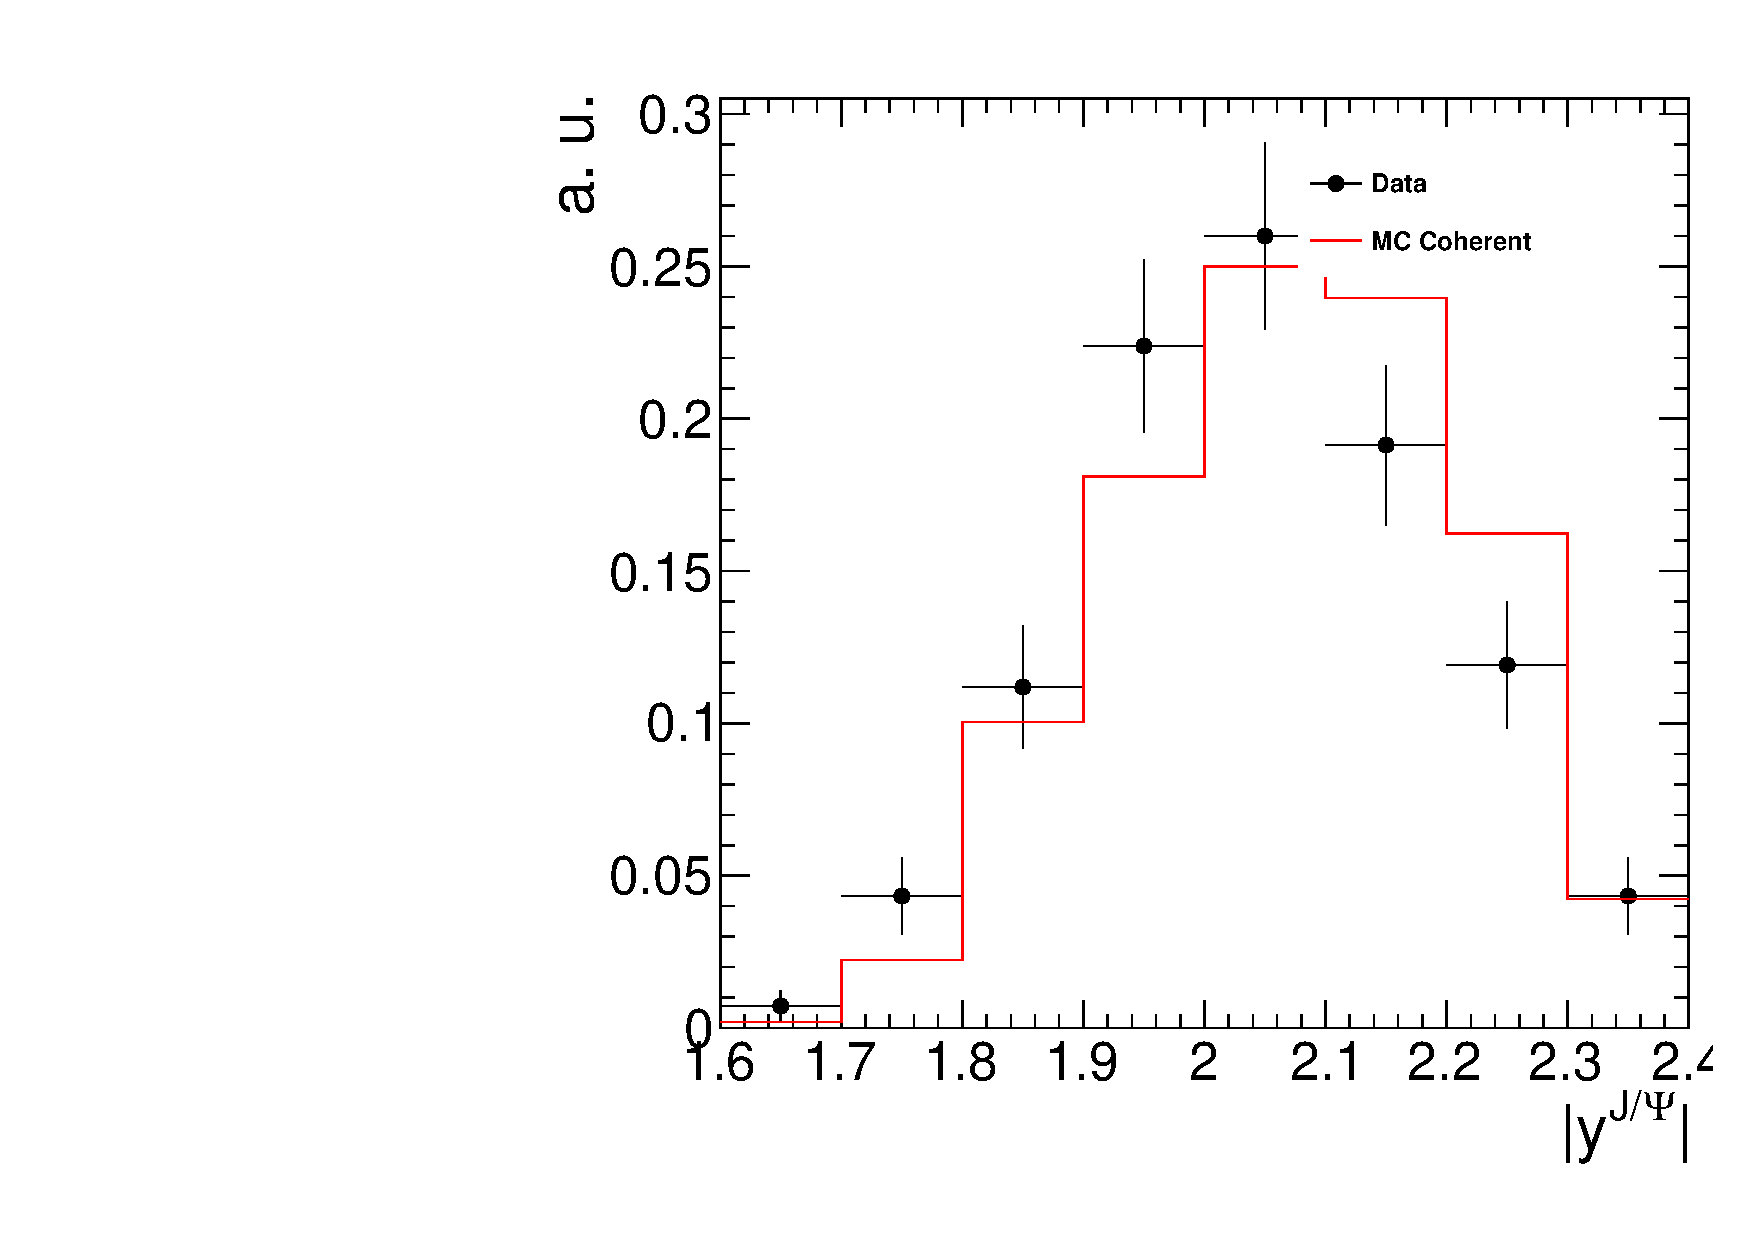
\includegraphics[width=0.5\textwidth]{jpsiMcComp/jpsiAbsRapCoherent}
      \caption{Comparison of the of the dimuon rapidity distributions between 
        coherent MC sample and Data.}
      \label{fig:jpsiAbsRapCoherent}
    \end{figure}
    \begin{figure}[h]
      \centering
      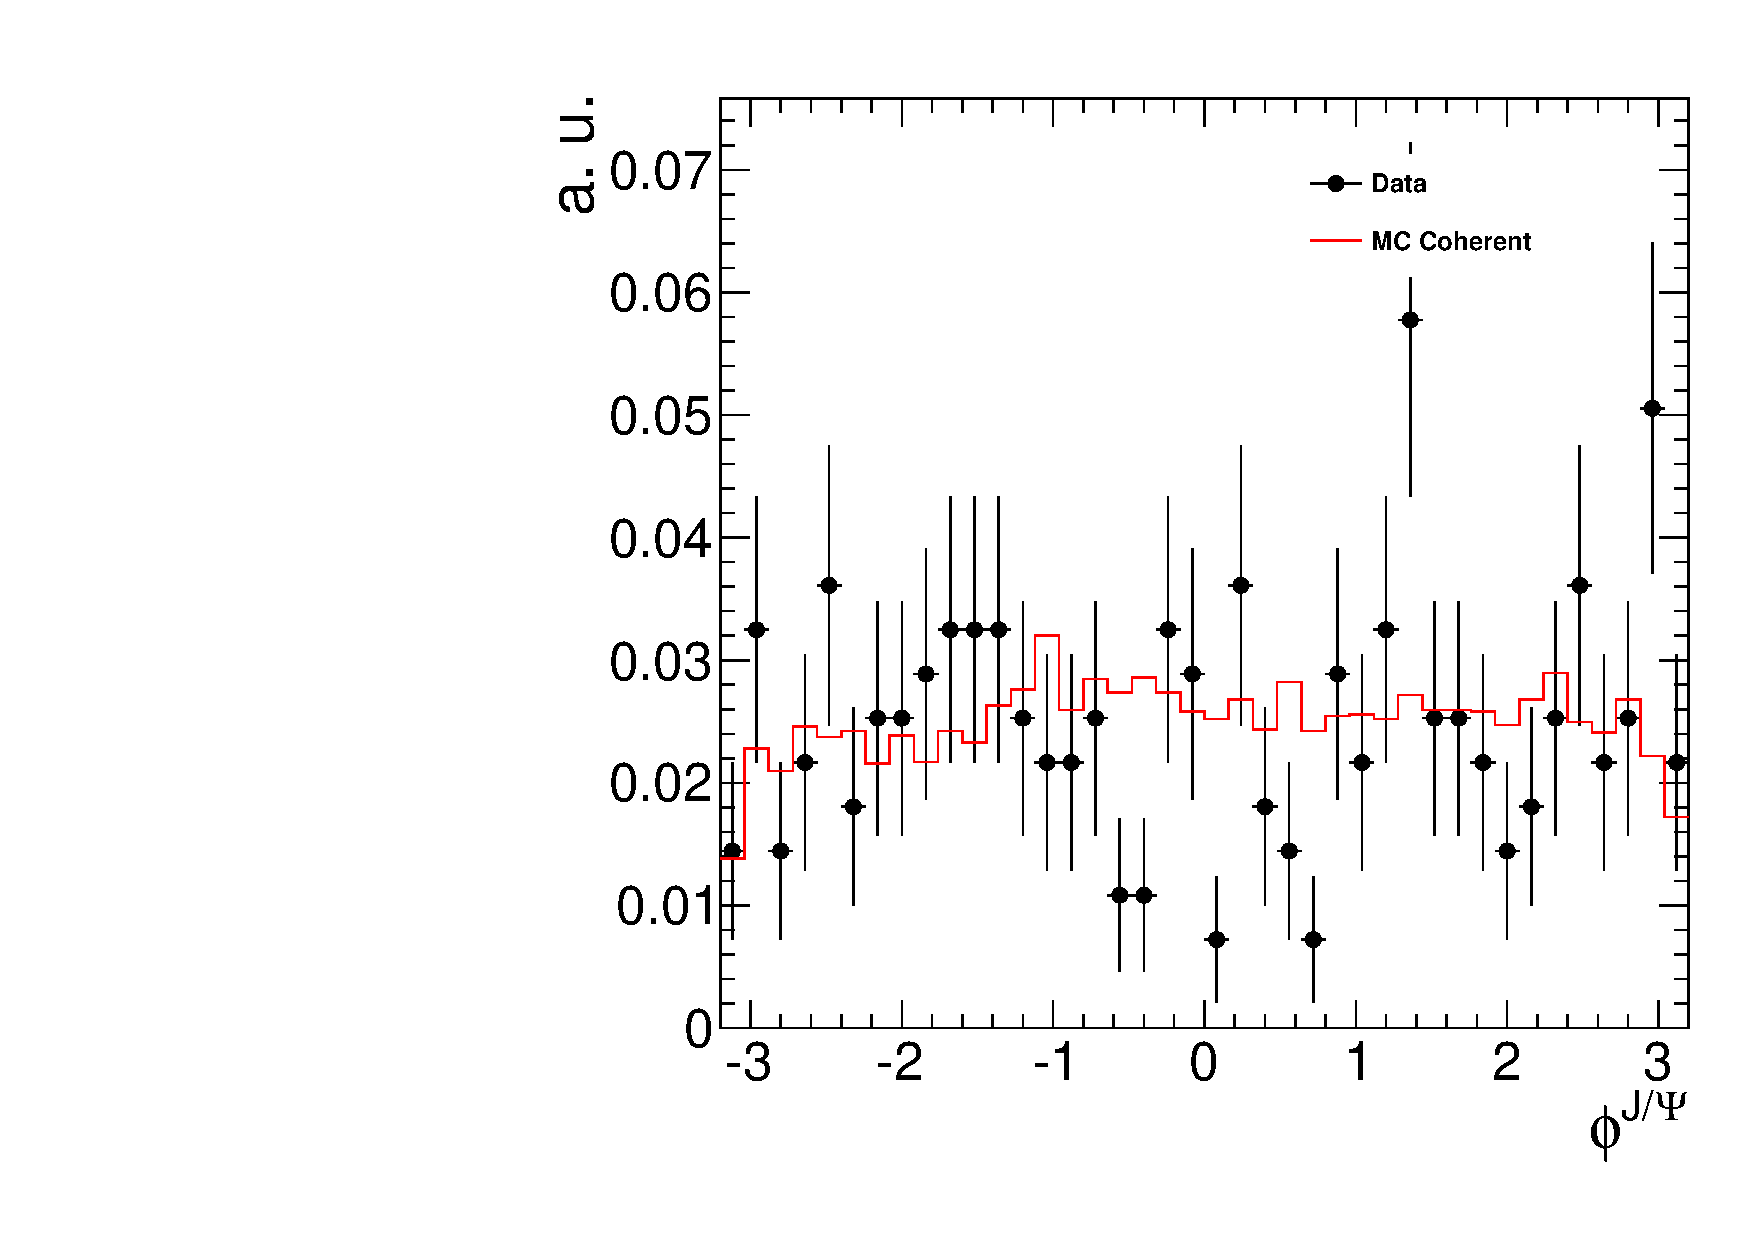
\includegraphics[width=0.5\textwidth]{jpsiMcComp/jpsiPhiCoherent}
      \caption{Comparison of the of the dimuon $\varphi$ distributions 
        between coherent MC sample and Data.}
      \label{fig:jpsiPhiCoherent}
    \end{figure}
    \begin{figure}[h]
      \centering
      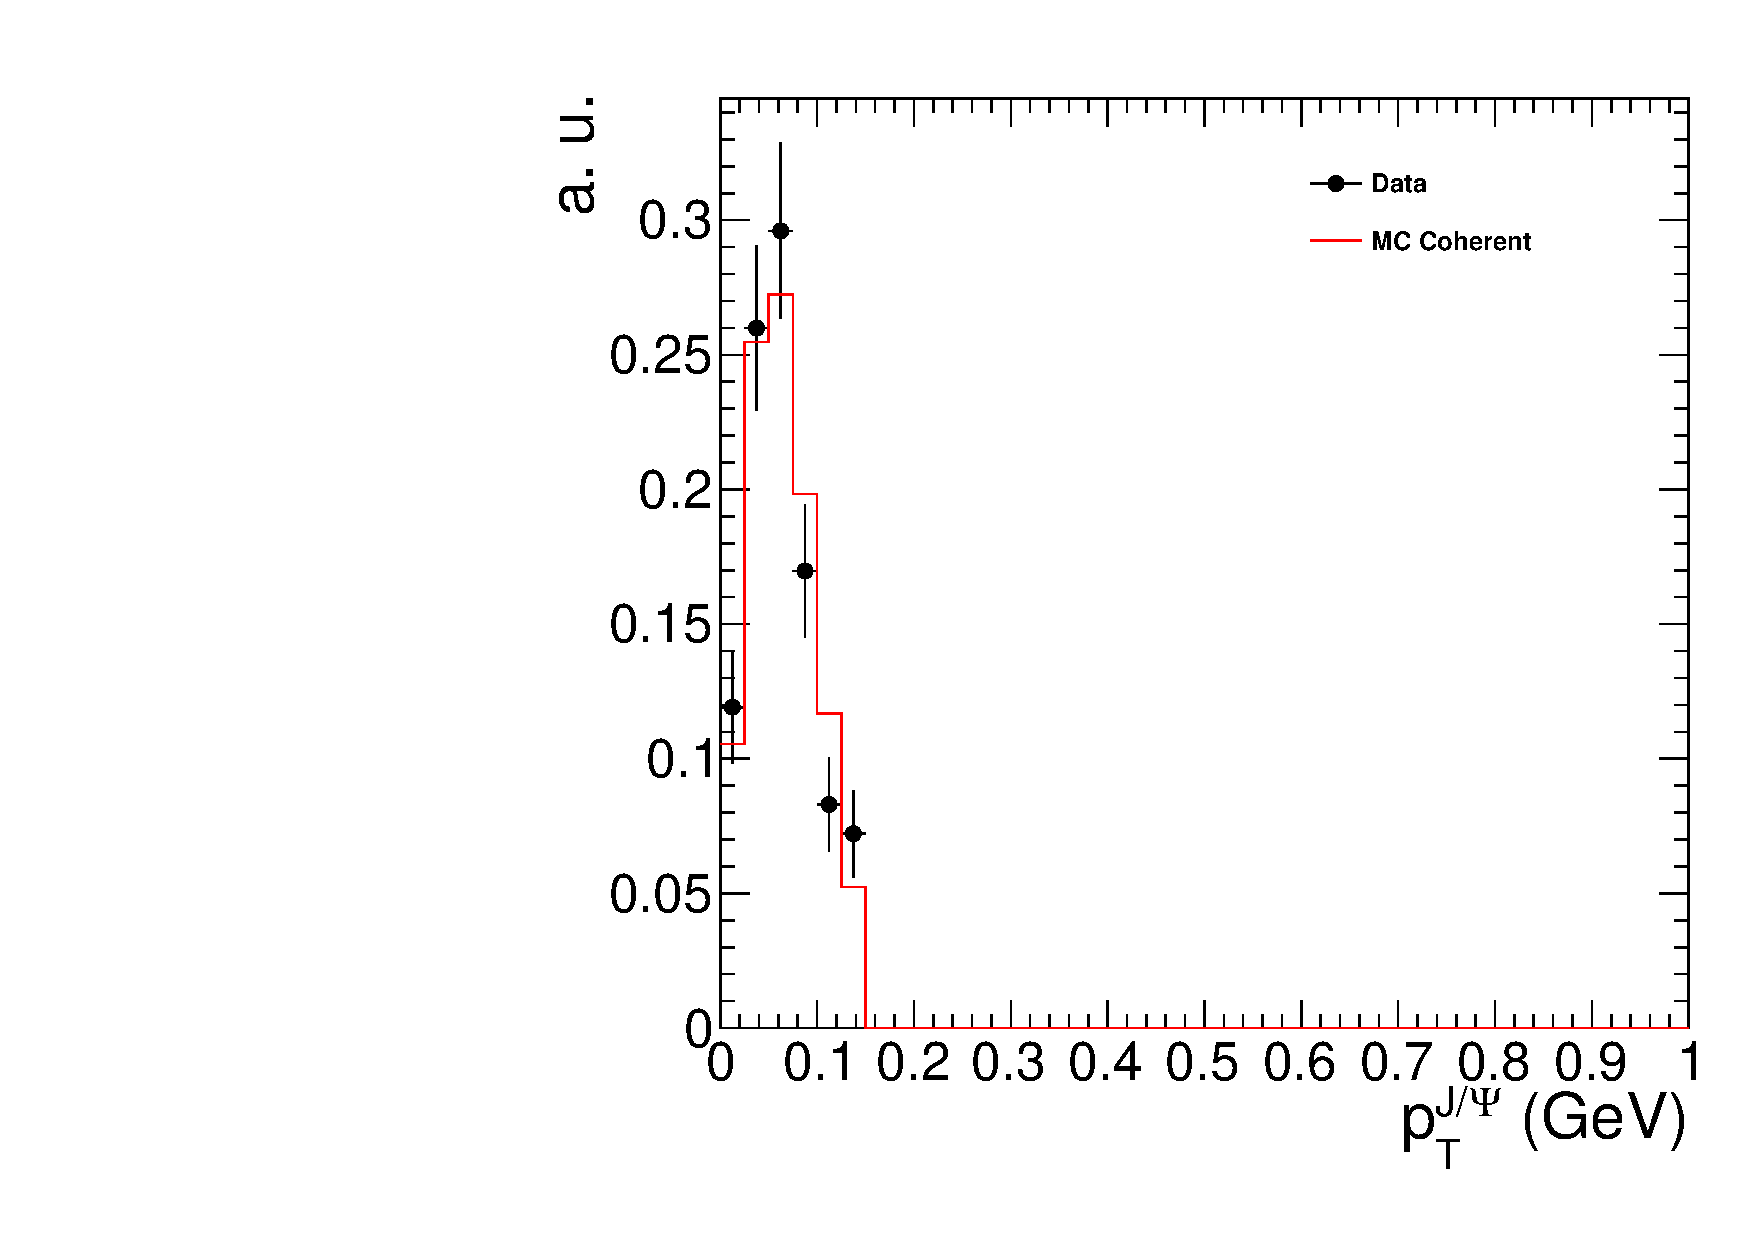
\includegraphics[width=0.5\textwidth]{jpsiMcComp/jpsiPtCoherent}
      \caption{Comparison of the of the dimuon p$_{\textrm{T}}$ distributions 
        between coherent MC sample and Data.}
      \label{fig:jpsiPtCoherent}
    \end{figure}

  \section{\label{sec:TrigDev} Trigger Development} 
    Prior to the 2011 LHC PbPb run, UPC events had not been directly studied in 
      PbPb collisions using CMS. 
    Design of the UPC triggers required studies of the 2010 data to estimate 
      rates and assure that the bandwidth used by these trigger would be
      sufficiently low. 
    All the different physics analyses must share the limited readout rate of 
      the detector.
    For this reason, conservation of bandwidth was a major design consideration.

    To estimate the 2011 rates prior to the run, the 2010 rates were used to 
      extrapolate to the interaction rate of the 2011 run. 
    The unique UPC triggers were estimated by combining existing triggers from
      the 2010 run. 
    By calculating the ratio between the UPC trigger rates and the minimum bias
      trigger rate, the UPC trigger rates were scaled up to the 2011 
      interaction rates using the 2010 data. 
    The extrapolated rates allowed for a package triggers to be created, which 
      fit within the bandwidth requirement of CMS Heavy Ions. 
    
    The trigger package for 2011 contained ZDC based efficiency monitoring 
      triggers, muon and electron based triggers for measuring $J/\psi$, and 
      backup triggers in case there was a problem with the original muon and 
      electron triggers.
    In order to recorded the trigger efficiency monitoring data, the ZDC 
      triggers had to be prescaled to a lower rate. 
    The scaling down of the monitoring triggers were setup to assure overlap
      with the signal triggers.
    By balancing the competing objectives of rate reduction and increasing 
      the overlap between the monitoring and signal triggers, 
      the prescales for the trigger were as seen in Table .%~\ref{triggerTabel2011}.

    \subsection{\label{sec:l1Trigger} L1 Trigger}
      The goal of the L1 triggers was to record enough data to measure dimuons
        and dielectrons in UPC events.
      To achieve this, the loosest muon trigger and lowest threshold ECAL 
        triggers where paired with a trigger on energy in the ZDC and a veto on
	    energy in the BSC or HF.
      The L1 package that was constructed for the analysis of UPC $J/\psi$ 
        is presented in Table~\ref{tab:l1Triggers2011}.

	\begin{table}[h]
		\centering
		\begin{tabular}{|l|l|}
		  L1 Trigger Seed  & Type \\ \hline \hline
		  L1\_MuOpen\_ZdcCalo\_NotBscMinBiasThresh2\_BptxAND & Physics \\  \hline
		  L1\_EG2\_ZdcCalo\_NotBscMinBiasThresh2\_BptxAND & Physics \\  \hline
		  L1\_EG5\_ZdcCalo\_NotBscMinBiasThresh2\_BptxAND & Physics \\ \hline
		  L1\_ZdcCaloMinus\_BptxAND & Monitor \\  \hline
		  L1\_ZdcCaloMinus\_BptxAND & Monitor \\  \hline
		  L1\_MuOpen\_ZdcCalo\_NotHcalHfCoincidencePm\_BptxAND & Backup \\ \hline
		  L1\_EG2\_ZdcCalo\_NotHcalHfCoincidencePm\_BptxAND & Backup \\ \hline
		  L1\_EG5\_ZdcCalo\_NotHcalHfCoincidencePm\_BptxAND & Backup \\ \hline \hline
		\end{tabular}
		\caption{List of 2011 L1 seeds.}
		\label{tab:l1Triggers2011}
	\end{table}
       
       The cumulative L1 trigger rate for all the UPC L1 trigger seeds was
         required to be 200 Hz.
       This requirement stemmed from the need to keep the tracker read-out rate
         low. 
       The trackers baseline voltage can fluctuate due to the high tracker hit 
         multiplicities in PbPb collisions.
       In order to monitor the zero suppression of the tracker, the zero 
         suppression algorithm was executed using the HLT computing farm 
	 rather than the in the tracker firmware. 
       The additional computing cycles needed to run the zero suppression 
         set the limit for L1 bandwidth. 

    \subsection{HLT Trigger}
      As opposed to the L1 trigger, which reads out the tracker, the HLT has 
        access to the tracker information. 
      Reconstruction of a track in the pixel detector is used by the UPC paths.
      The use of the pixel detector only, as opposed to using the whole tracker 
        including the silicon strip detector, allows for quick track 
	reconstruction saving computing cycles.
      The requirement of at least on reconstructed pixel track for the HLT 
        triggers was designed to reject backgrounds where no particles are 
	reconstructed by the tracker. 
  \begin{table}[h]
		\centering
		\begin{tabular}{|l|l|}
		  \hline HLT Trigger  \\ \hline \hline
		  HLT\_HIUPCNeuMuPixel\_SingleTrack & Physics   \\ \hline
		  HLT\_HIUPCNeuEG2Pixel\_SingleTrack & Physics   \\ \hline
		  HLT\_HIUPCNeuEG5Pixel\_SingleTrack & Physics   \\ \hline
		  HLT\_HIMinBiasZDC\_Calo\_PlusOrMinus\_v1  & Monitor  \\ \hline
		  HLT\_HIMinBiasZDC\_PlusOrMinusPixel\_SingleTrack\_v1   & Monitor \\ \hline
		  HLT\_HIUPCNeuHcalHfMuPixel\_SingleTrack & Backup   \\ \hline
		  HLT\_HIUPCNeuHcalHfEG2Pixel\_SingleTrack & Backup   \\ \hline
		  HLT\_HIUPCNeuHcalHfEG5Pixel\_SingleTrack & Backup   \\ \hline \hline
		\end{tabular}
		\caption{List of 2011 HLT trigger.}
		\label{tab:hltTriggers2011}
	\end{table}

	The total HLT output for the UPC trigger paths was 20 Hz. 
	The limiting factor for the HLT rate was the amount of disk space 
	  available to store the data. 

  \section{\label{sec:DataSetEvSel} Data Sets and Event Selection}
    \subsection{Data Set}
      In order to investigate novel physics processes like UPC $J/\psi$ 
       production, the LHC has delivered unprecedented amounts of data.
      The data for this analysis was recorded during the 2011 LHC PbPb run. 
      During this period, 157 $\mu$$b^{-1}$ where recorded by the CMS detector,
        corresponding to over a billion PbPb collisions. 
      Of this, 143 $\mu$$b^{-1}$ are used in this analysis.
  
      Three specially selected samples are used (see Table~\ref{tab:sampleLumiNevt}).
      These samples were recorded using subsets of the triggers found in 
        Section~\ref{sec:TrigDev}.
      The $J/\psi$ events discussed in this thesis were obtained analyzing the 
      sample labeled in Table~\ref{tab:sampleLumiNevt} as physics.
      A minimum bias sample was recorded for the sake of estimating efficiencies.
      Last, a zero bias sample was recored for investigating the ZDC and the 
        noise distributions of HF.
      By recording this hierarchy of samples, interesting events are selected 
        with a much higher purity in the physics sample, while the zero bias and 
        minimum bias samples allow for the investigation of the selection 
        criteria. 
  
      To record the physics sample containing the $J/\psi$ signal, a muon trigger
        was paired with a veto on energy in the BSC and a requirement that there 
        be energy in at least one of two sides the ZDC. 
      This trigger utilizes the unlikely chance of having overlapping noise in
        in the ZDC and muon detector.
      Because of the characteristically low momentum of UPC $J/\psi$ as compared
        to $J/\psi$ created by other physics process, the loosest muon 
        trigger was used.
      The trigger rejects muon noise by requiring that a interaction took place
        that deposits energy in the ZDC.
      Contributions from hadronic interactions are reduced by the veto on the 
        BSC.
      In this way the balance between reducing the rate and maximizing the 
        efficiency was struck, allowing for the data to be recorded without 
        producing high rates resulting in dead time for the detector.  
      
      In order to investigate the muon trigger and the other parts of the events 
        selection, a minimum bias sample was recorded using the ZDC. 
      For ZDC triggered sample, any event which had energy consistent with at 
        least one neutron in either of the two sides of the ZDC was recorded.
      This process is much more common than the UPC $J/\psi$ production.
      For this reason, the rates of this trigger are much higher than the physics
        trigger, and only a small sub set of these events are recorded.
      From this trigger the pixel track efficiency was estimated. 
  
      In addition to the minimum bias and physics sample, a zero bias sample was 
        recorded to examine the ZDC trigger and the HF noise distributions. 
      The zero bias trigger fired every time both beams passed through CMS. 
      Only 4 events out of every million triggered were recorded for this sample. 
      This sample allowed for an unbiased measurement of the ZDC trigger 
      efficiency as discussed in Section~\ref{sec:effDet}. 
      Because the zero bias trigger does not require any activity in any of the
        CMS sub detectors, the sample contains very few hadronic collisions. 
      This allowed for a measurement of the electronic noise distributions in
        the HF, which will be discussed in the next section.
  
      The integrated luminosity for each of the three samples is calculated
        by recording activity in HF. 
      The cross section for HF activity is measured from a van der Meer scan, and
        the cross section was found to be \textcolor{red}{X}.
      In this way the amount of integrated luminosity for any period running is
        related to the activity in HF. 
      \begin{table}
  	    \centering
  	    \begin{tabular}{|l|l|l|}
  	      \hline Sample & Events & $L_{int}$ \\ \hline \hline
  	      Physics & \textcolor{red}{300K} & \textcolor{red}{143.3 
  	        $\mu$$b$} \\ \hline
  	      Minimum Bias & \textcolor{red}{100K} & \textcolor{red}{X} \\ \hline
  	      Zero Bias & \textcolor{red}{5M} & \textcolor{red}{580 b} \\ \hline \hline
  	    \end{tabular}
  	    \caption{Integrated luminosities and number of events for the three
  	      samples used in this analysis.}
  	    \label{tab:sampleLumiNevt}
      \end{table}
      An additional method was used to cross check the integrated luminosity 
        obtained by the van der Meer scan technique.
      The integrated luminosity can also be measured by counting the events that
        fire the L1 minimum bias trigger together with the inelastic PbPb cross 
        section. 
  
    \subsection{Event selection}
      The analysis described in this thesis focuses on UPC $J/\psi$s decaying to 
        muons. 
      The trigger used for this analysis recored \textcolor{red}{X} events.
      A set of off-line cuts were applied to increase the relative contribution 
        of UPC events relative to background processes. 
      The following cuts were applied. 
  
      Two sets of event selection cuts are applied to reject background events. 
      The first set rejects background from the beam.
      The second reject events where hadronic collisions have occurred.
      
      To reject beam induced background the following cuts were applied:
      \begin{itemize}
        \item The reconstructed vertex must be within \textcolor{red}{X} cm in 
          the transverse direction and \textcolor{red}{X} cm in the 
          longitudinal direction. This cut assures that reconstructed particles 
          come from interactions between the two beams rather than event where 
          one of the two beams interact with gas particles near the interaction 
          point. 
  	    \item Beam halo muons were rejected using the timing of the muon hits.
              The beam halo cut rejects events where muons surrounding the beam 
              stream through the detector. 
  	    \item Pixel cluster shape should be compatible with the vertex. 
          This cut requires that energy deposits in the silicon tracker point 
            back to the reconstructed  primary vertex. 
      \end{itemize}
      These beam background cuts do not reject any UPC $J/\psi$ candidates. 
  
      The second set of background rejection cuts were designed to 
        reduce contamination from hadronic interactions. 
      \begin{itemize}
  	    \item No more than 2 reconstructed tracks in the event.
          The track requirement rejects events that produce many charged 
          particles.
  	    \item Maximum reconstructed hit energy in HF was required to be below 
            the threshold for electronic noise. 
          Nearly all hadronic interactions ($\sim$ 98\%) produce particles in the 
            range $3<|\eta|<5$ covered by the HF detector.
          By requiring that the energy deposits in HF resemble noise, nearly all
            elastic hadronic collisions are expected to be rejected.
  	    \item Energy in the ZDCs consistent with neutrons on only one side 
            of the interaction point
          In hadronic interactions both nuclei break-up. 
          By requiring that ZDC only reconstruct neutrons on one side of the 
            interaction point, hadronic interactions that produce neutrons on both 
            sides were rejected.
      \end{itemize}
      Each of these cuts are designed to reject topologies produced by hadronic
        interactions.
      The effect of these cuts can be seen in Table\textcolor{red}{X}.
  
      The following standard muon quality cuts are applied:
      \begin{itemize}
        \item Tracker track matched with at least one muon segment 
          (in any station) in both X and Y coordinates (< 3 $\sigma$).
        \item Cut on number of tracker layers with hits $>$ 5.
        \item Number of pixel layers $>$ 0.
        \item The $\chi^{2}$ per degrees of freedom of the track fit $<$ 3. 
        \item Loose transverse and longitudinal impact parameter cuts, with in 3 
          cm in the transverse direction and withing 30 cm in the longitudinal 
          direction with respect to the primary vertex.
      \end{itemize}
       These cuts are applied to reduce the number of fake muons.
  
  \section{break up determination}
    \subsection{ZDC Signal Reconstruction}
      There are 18 zdc channel. 
      There are 4 hadronic channels and 8 electromagnetic channels on each side
        of the CMS. 
      To measure neutrons in the ZDC the charge in each channel is first 
        converted to a signal. 

	\begin{figure}[h]
		\centering
		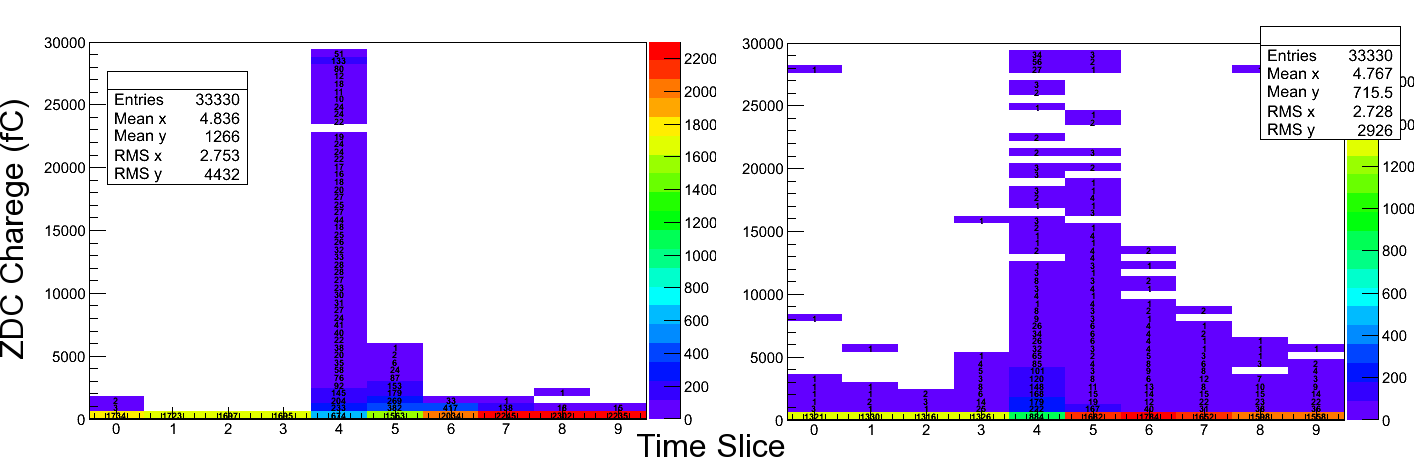
\includegraphics[width=\textwidth]{zdcPulseShape}
		\caption{ZDC pluse shape.}
		\label{fig:zdcPulseShape}
	\end{figure}

      Channel Signal definition:
      The signal in the zdc calculated two ways. 
      \begin{enumerate}
	\item Method 1
	\begin{enumerate}
	  \item signal: 4,5,6 
          \item background: 1,2
        \end{enumerate}
	\item Method 2
	\begin{enumerate}
	  \item signal: 4
	  \item background: 5
        \end{enumerate}
      \end{enumerate}

      As seen in Fig~\ref{fig:zdcPulseShape}, method 1 uses all the dominant 
        signal time slices and uses the maximum number of “clean” non signal 
        time slices to estimate the noise pedestal event by event. 
      This minimizes the effect of random noise time slice by time slice by 
        averaging over the maximum number of time slices per event. 

      Method 2 uses only the two time slice that are most likely to be above 
        zero. 
      Because all signal that is less than zero is not measured, method 1 
        only allows for a noise pedestal measurement half the time.
    
      From these two methods the ZDC+ and ZDC- energy spectra near the 
        one neutron peak are plotted in Fig.~\ref{fig:zdcSpec2v1}.
      While method 1 in blue and method 2 in reddo not differ much in ZDC-, 
        the clear separation of the one neutron peak signal from the noise 
        peak about zero is evident. 
      \begin{figure}[h]
        \centering
        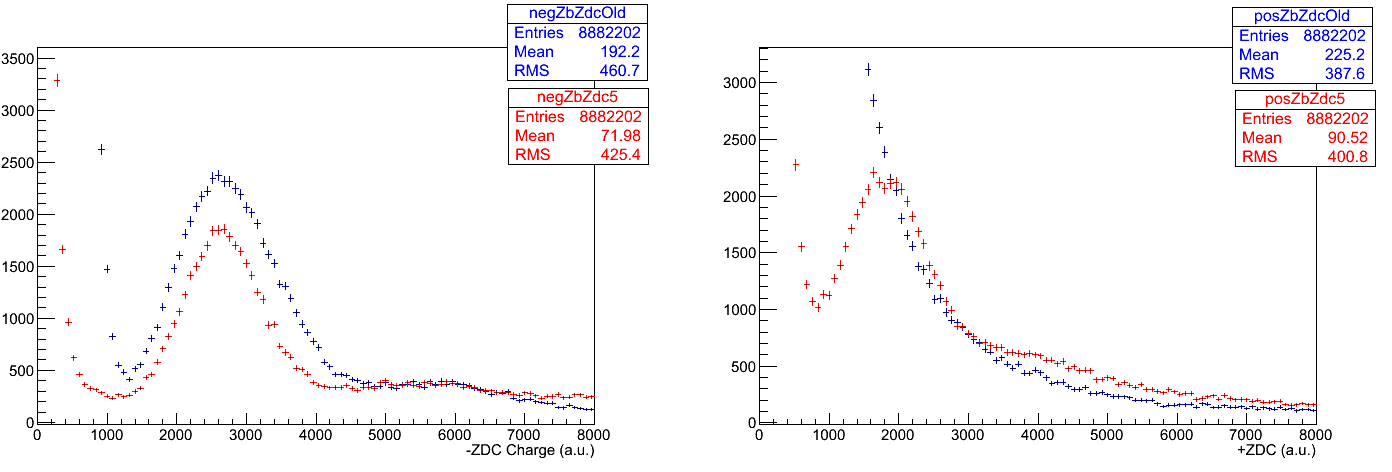
\includegraphics[width=\textwidth]{zdcSpec2v1}
        \caption{Comparison of ZDC signal reconstruction methods.}
        \label{fig:zdcSpec2v1}
      \end{figure}

    \subsection{Determination of the one neutron thresholds}
      The ZDC thresholds used to establish the break-up mode were measured from
        zero bias data.
      By using this dataset, the spectrum does not contain a trigger bias. 
      The trigger requriment in the event is that both beams were present in 
        CMS.
      This does however include a significant electronic noise contribution due
        to events where no neutrons are emitted in the direction of the zdc.
      To sperate the signal from the electronic noise additional cuts are 
        applied in the zero bias data.

      In Fig.~\ref{fig:zdcPulseShape} the pulse shape peaks in the peaks in the
        fourth time slice, for electronic noise however, any of the ten time 
        slices are equally likely to have a peak value.
      Using this fact, signal can be preferably selected by requiring that the
        hadronic channels of the ZDC have a peak signal in the fourth time 
        slice.
      \begin{figure}[h]
        \centering
        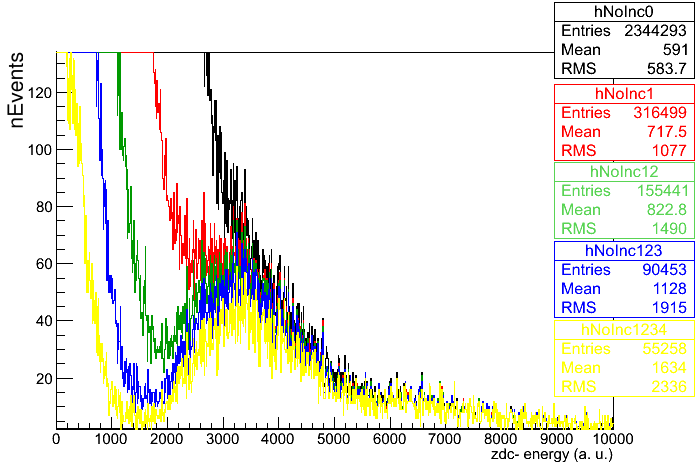
\includegraphics[width=0.6\textwidth]{zdcMinusSingleNuNoInc}
        \caption{Effects of requiring in time signal in ZDC hadronic 
          channels.}
        \label{fig:zdcTimingCuts}
      \end{figure}
      In Fig.~\ref{fig:zdcTimingCuts} no noise subtraction is used. 
      As each additional hadronic channel is required to have a maximum signal
        in the fourth time slice, the single neutron peak emerges. 
      Using the noise subtraction method described by Method 1, same signal
        emerges.
      \begin{figure}[h]
        \centering
        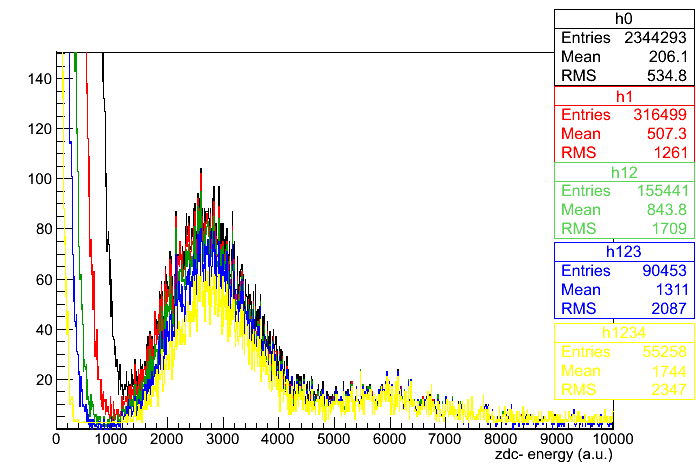
\includegraphics[width=0.6\textwidth]{zdcMinusSingleNuNoSub}
        \caption{Effect of ZDC signal timing requirements after noise 
          subtraction.}
        \label{fig:zdcTimingAfterNoiseSub}
      \end{figure}
      Fig.~\ref{fig:zdcTimingAfterNoiseSub} confirms that both noise 
        subtraction and the timing require produce the same signal.
      This gives confidence that the signal is not an artifact of either cut, 
        but the true neutron signal. 

  \section{Signal extraction}
    The invariant mass distribution for opposite sign dimuons is shown in 
      Figure~\ref{fig:massFit}. 
    A J/$\psi$ signal is clearly visible together with tails at higher and lower mass
      due to the photon-photon process
    A fit to the invariant mass distribution was done using a Gaussian and a Crystal Ball
      function to account for the J/psi signal and a first and second order polynomial 
      function for the photon-photon process.
    The extracted number of J/$\psi$ candidates from this fit includes all J/$\psi$s in
      the mass window that pass the analysis cuts. 
    
    The p$_{T}$ spectrum is fit using templates from the three physics MC samples. 
    These contributions display a different shape in transverse momenta. 
    For this reason, the number of coherent J/psi candidates were extracted 
      from the dimuon Pt distribution, around the J/psi mass, after fitting 
      together MC templates for both signal and background.

      \begin{figure*}[!Hhtb]
        \centering
        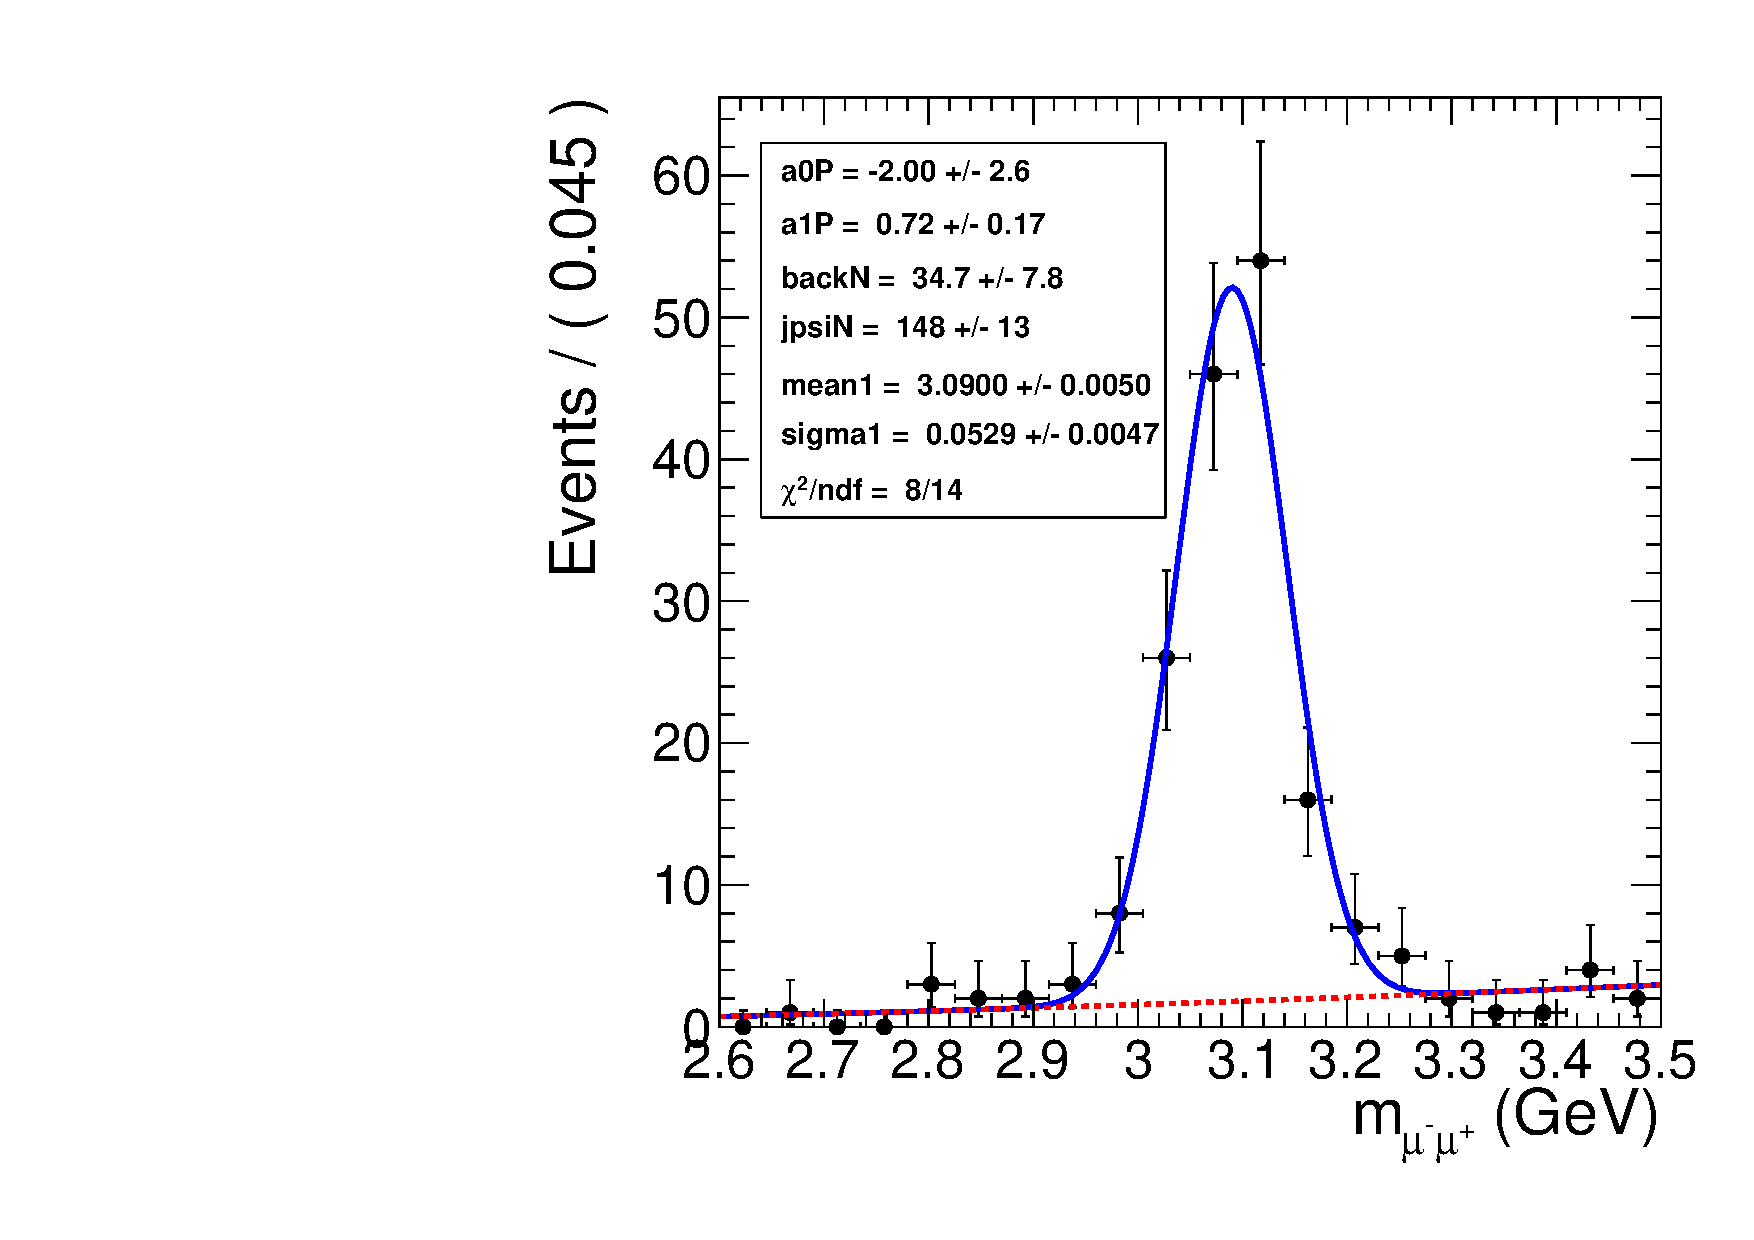
\includegraphics[width=.45\textwidth]{massFitSimple}
        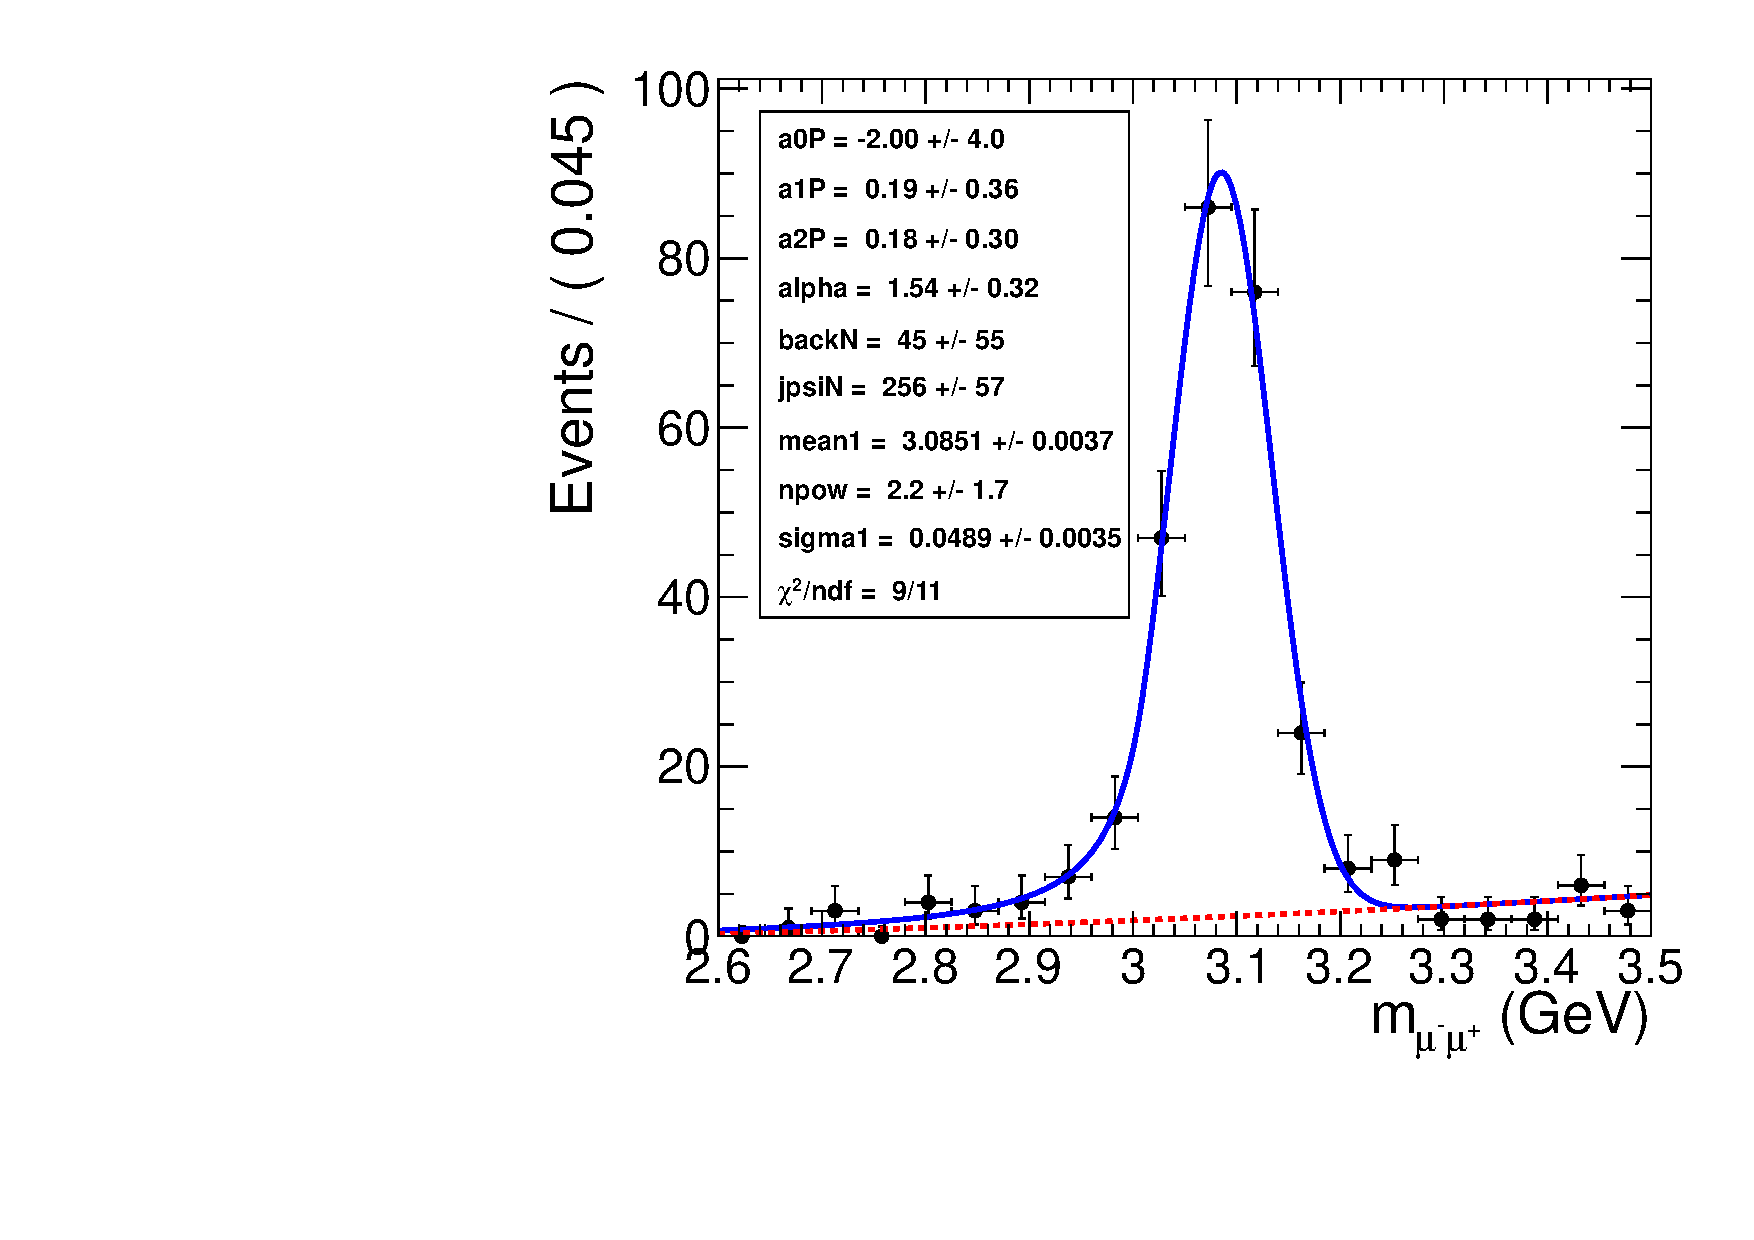
\includegraphics[width=.45\textwidth]{massFitCBPoly2}
        \caption{Mass fit to J/$\psi$ using Gaussian (Left) and Crystal Ball (Right) for the 
          signal and a polynomial for the background}
        \label{fig:massFit}
      \end{figure*}

      \begin{figure}[!Hhtb]
        \centering
        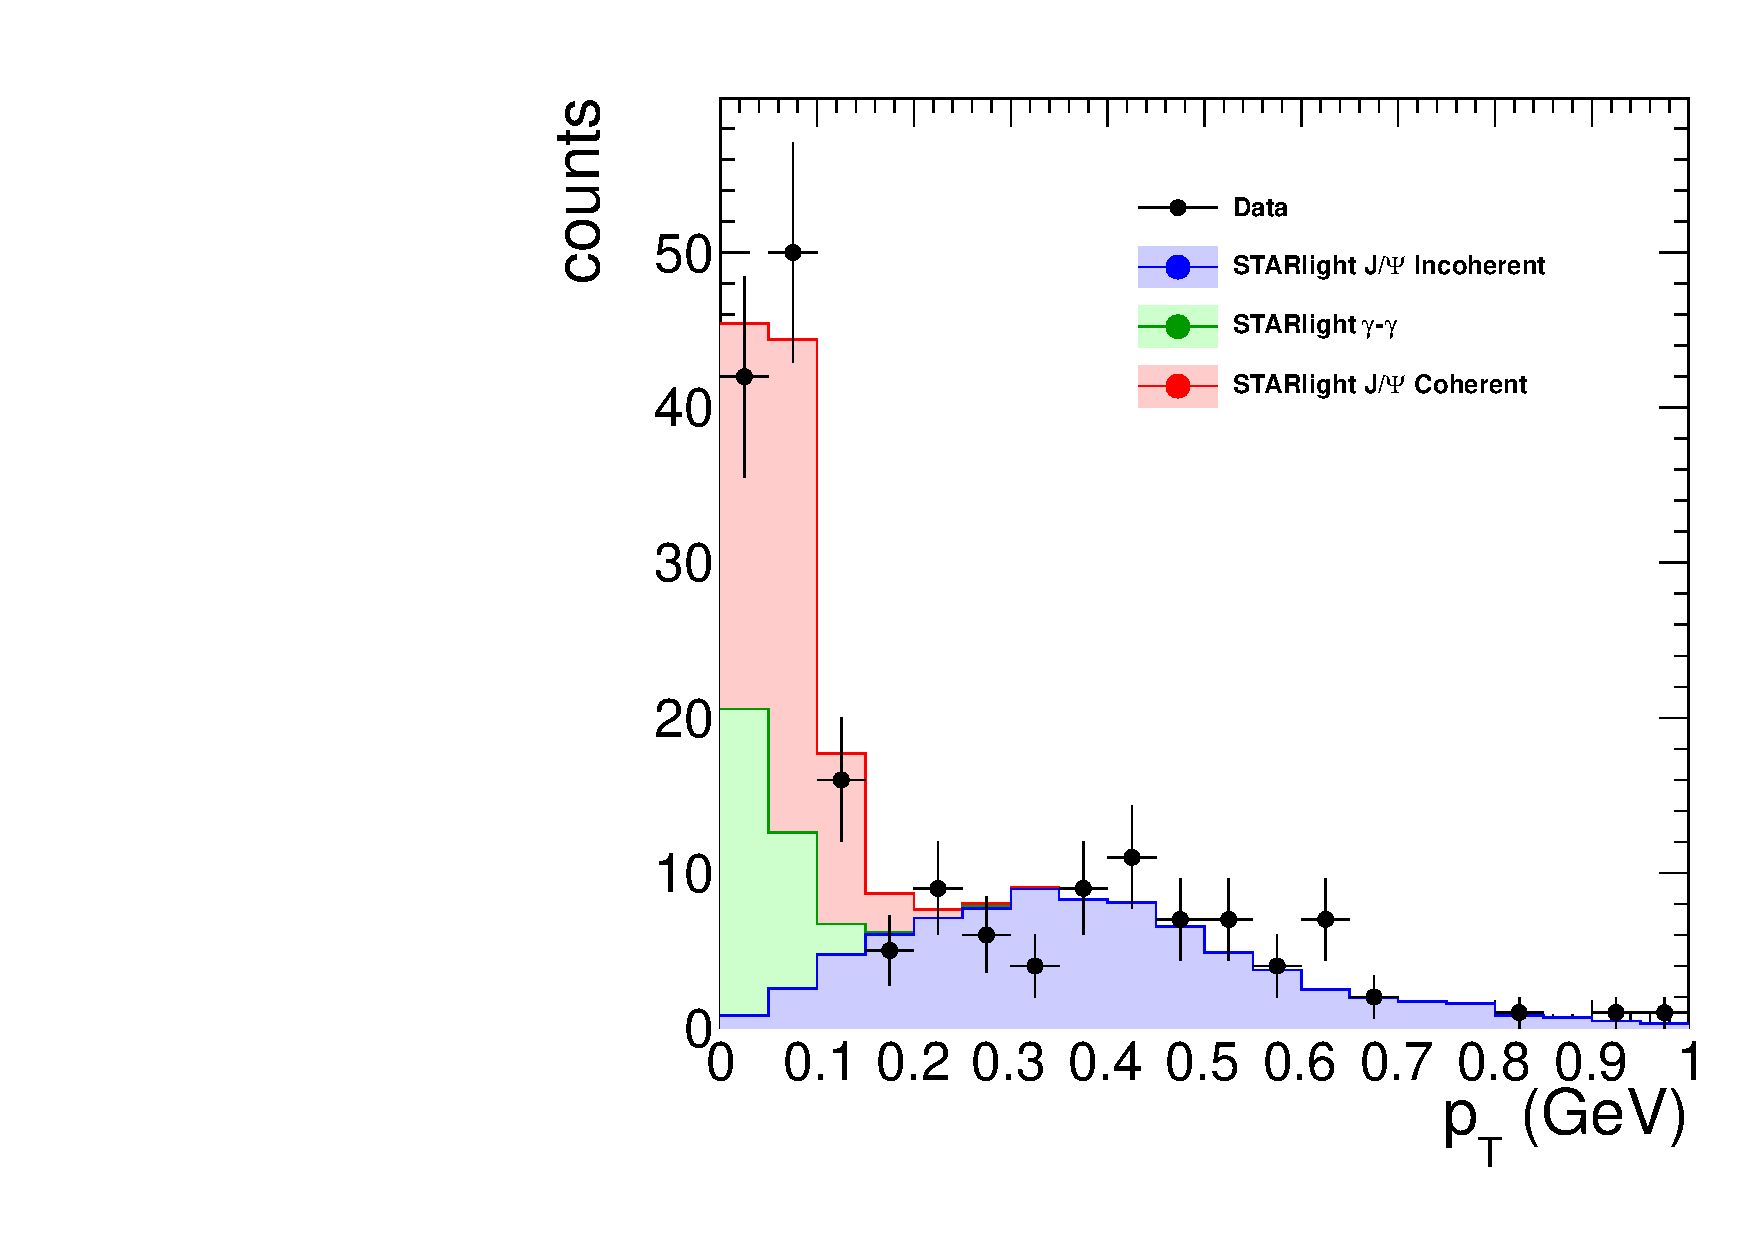
\includegraphics[width=.6\textwidth]{ptTemplateFit}
        \caption{Coherent, incohernt, and photon-photon process p$_{T}$ template fit to data.}
        \label{fig:ptTempFit}
      \end{figure}

  \section{\label{sec:effDet} Efficiency determination}
    \subsection{Muon Efficiencies}
      The muon efficiencies are measured from M.C and data.
      The M.C. based measurement accounts for the detector acceptance and the 
        efficiency of the muon quality discussed in 
        Section~\ref{sec:DataSetEvSel}.
      The trigger efficiencies were measured by tag and probe.
      
      To measure the detector acceptance, the muon daughter reconstruction 
        efficiency is measured.
        $\varepsilon^{\mu}_{reco} = \frac{N^{\mu}_{reco}}{N^{\mu}_{gen}}$
        \begin{figure*}[!Hhtb]
          \centering
          $ \begin{array}{cc}
            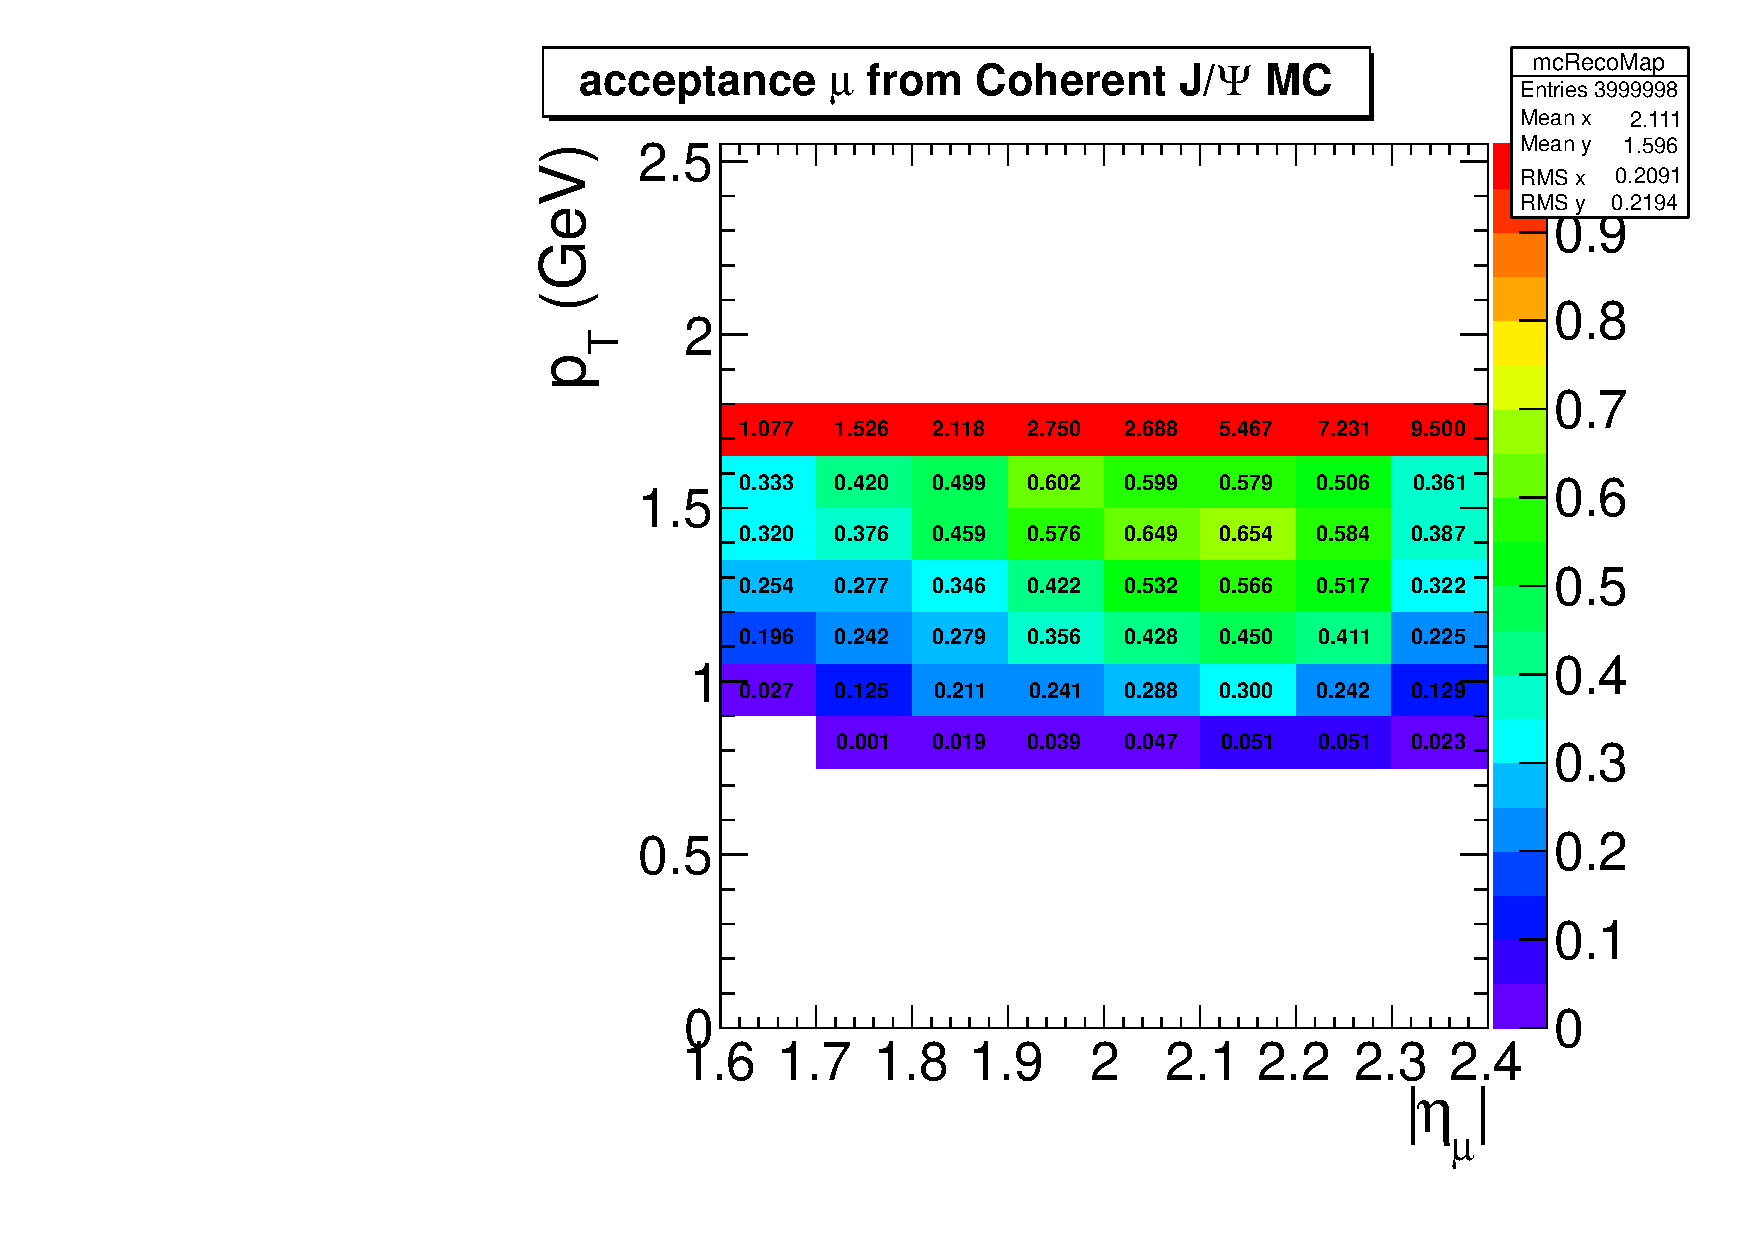
\includegraphics[width=.45\textwidth]{mcEffMaps/accMuJpCo} &
            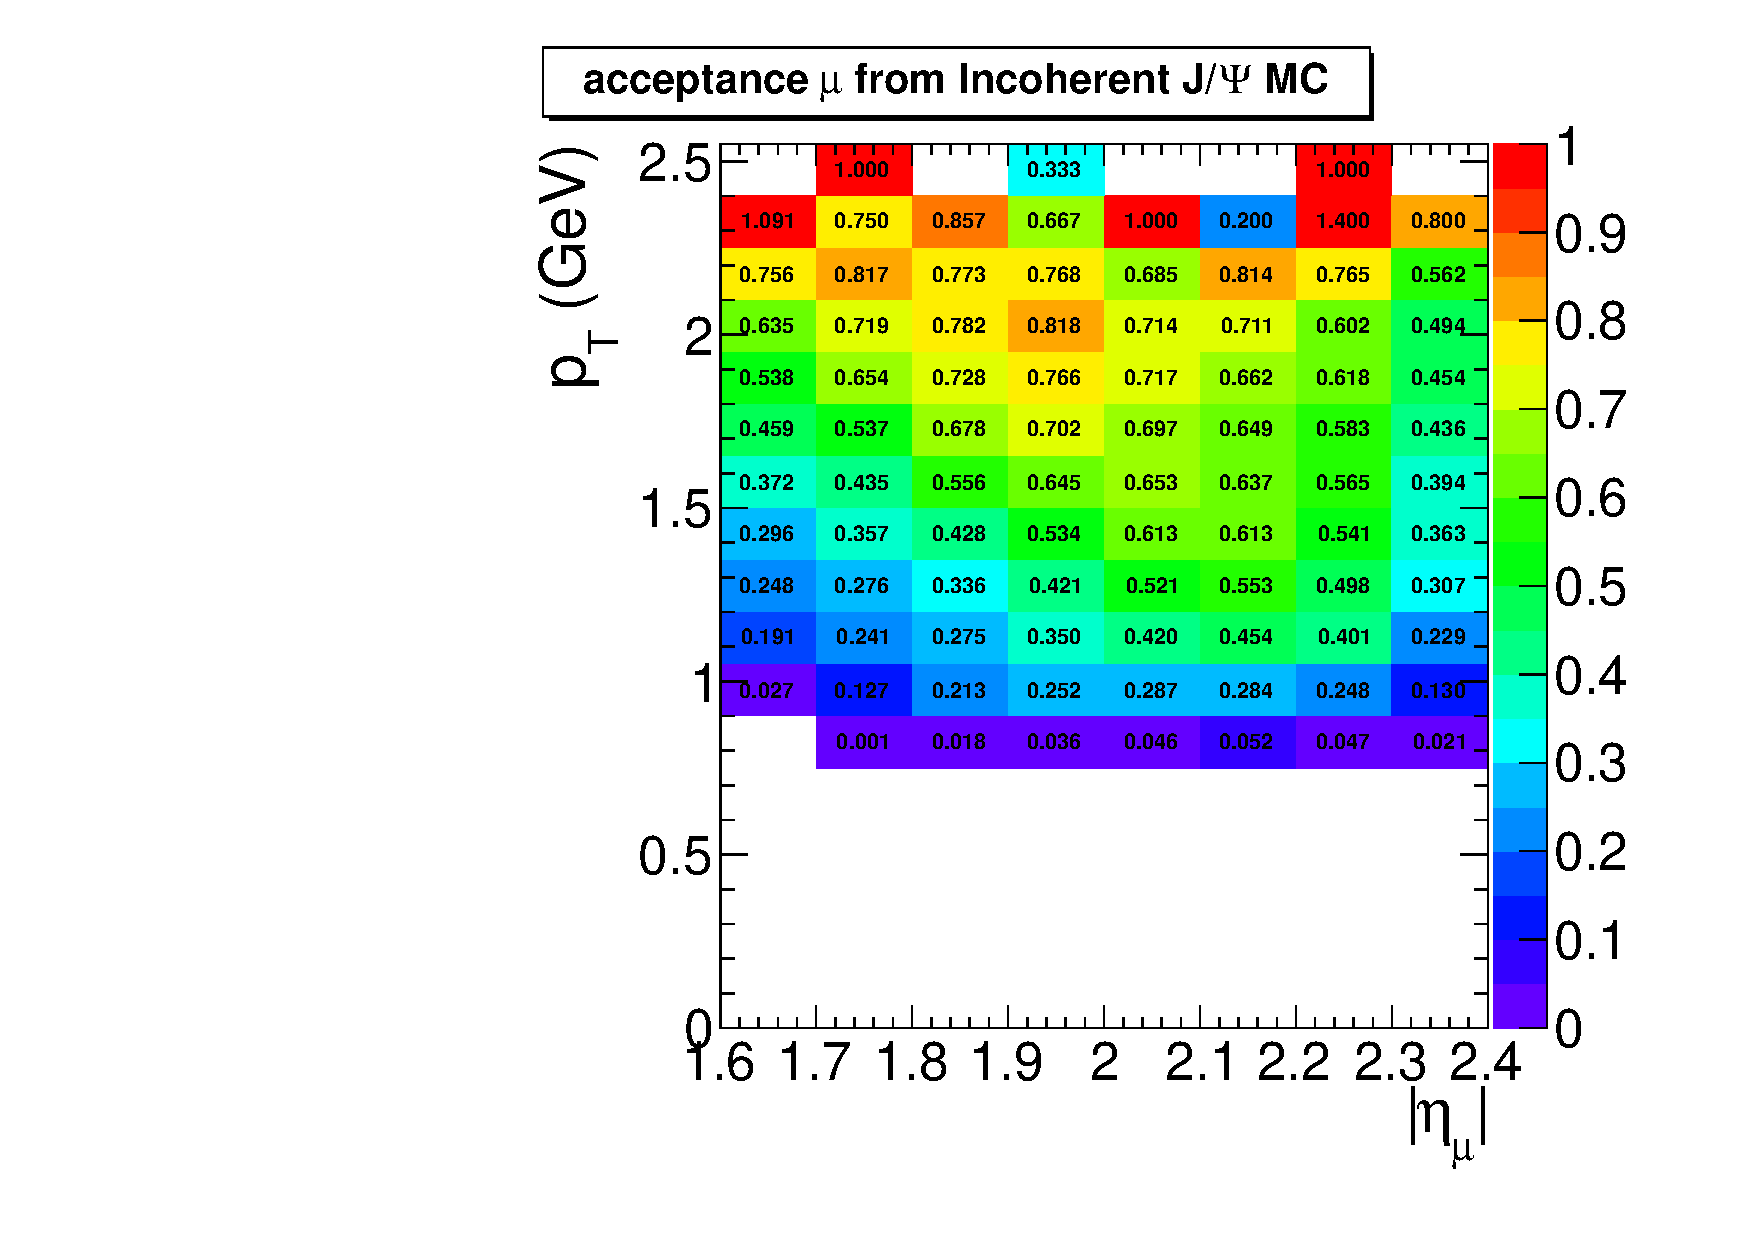
\includegraphics[width=.45\textwidth]{mcEffMaps/accMuJpInCo} \\
            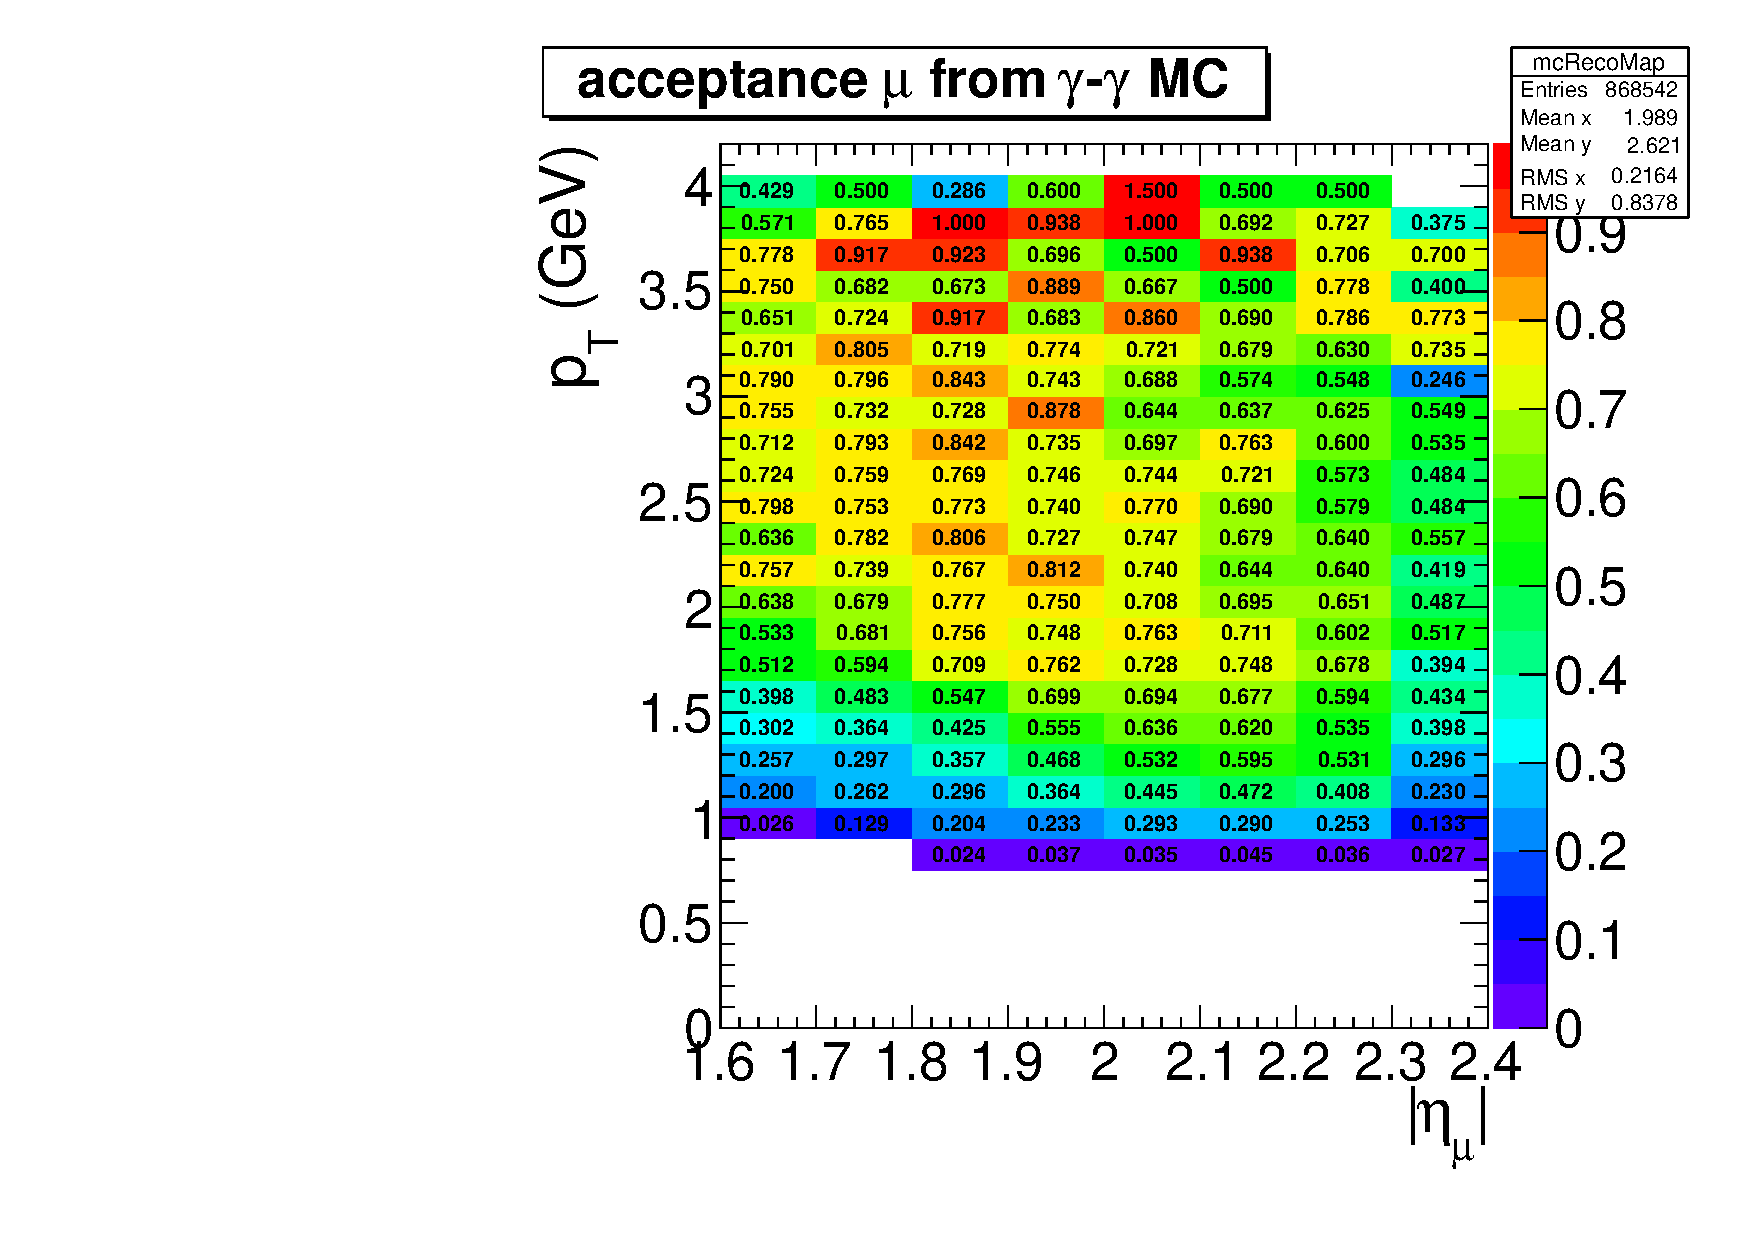
\includegraphics[width=.45\textwidth]{mcEffMaps/accMuGamma} &
            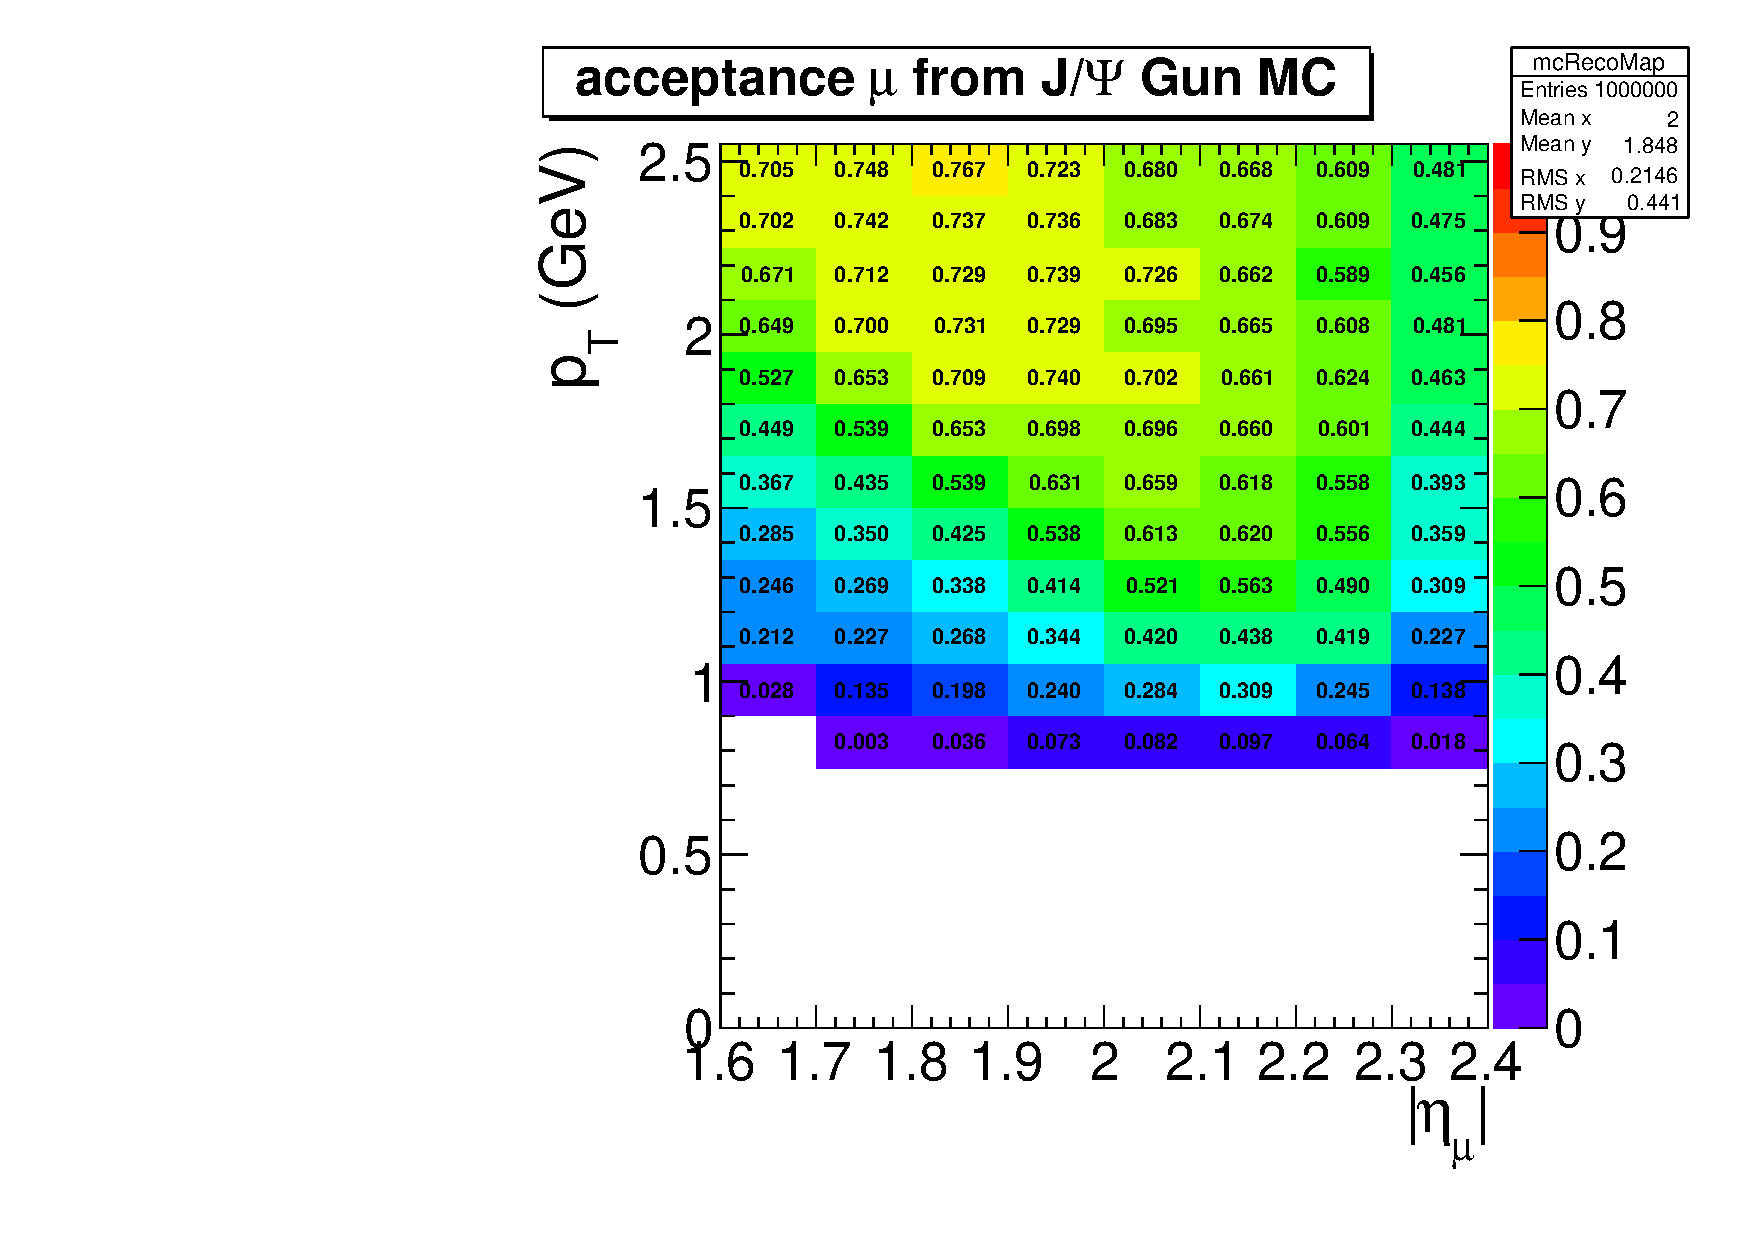
\includegraphics[width=.45\textwidth]{mcEffMaps/accMuGun}
          \end{array} $
          \caption{ Muon daughter detectability from coherent J/$\psi$, 
            incoherent J/$\psi$, photon-photon, and J/$\psi$ gun samples.}
          \label{fig:muonDaughterDet}
        \end{figure*}
      Muon daughter detectability cuts were established from 
        Fig.~\ref{fig:muonDaughterDet}.
      All muons that were reconstructed with an efficiency better than 20\% 
        were declared detectable.
      Fig.~\ref{fig:muonDaughterDet} shows that reconstruction of the muon 
        daughters does not depend on the generator used.
      The ability to reconstruct a muon depends only on the detector. 

      CMS has a limited acceptance for $J/\psi$s. 
      This is particularly the case for $J/\psi$s with low momentum like those
        produced in UPC events. 
      To measure the CMSs acceptance for $J/\psi$, reconstructed dimuon 
        candidates were considered detectable if both reconstructed daughters 
        in fell into the 20\% detectability region defined by 
        Fig.~\ref{fig:muonDaughterDet}.
      The acceptance of the reconstructed dimuons are calculated from MC in 
        using the following formula:
      \begin{equation}
        A=\frac{N_{detectable}(y,p_{T})}{N_{gen}(y,p_{T})}
        \label{eq:jpsiAccEq}
      \end{equation}
      From Eq.~\ref{eq:jpsiAccEq}, the acceptance for $J/\psi$ was calculated
        as a function of y, and p$_{T}$ (see Fig.~\ref{fig:jpsiAcceptance}).
        \begin{figure*}[!Hhtb]
          \centering
          $ \begin{array}{cc}
            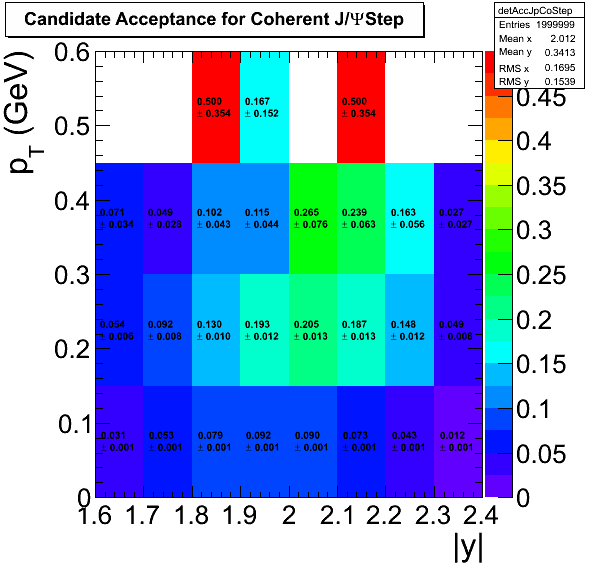
\includegraphics[width=.45\textwidth]{mcEffMaps/detAccJpCoStep} &
            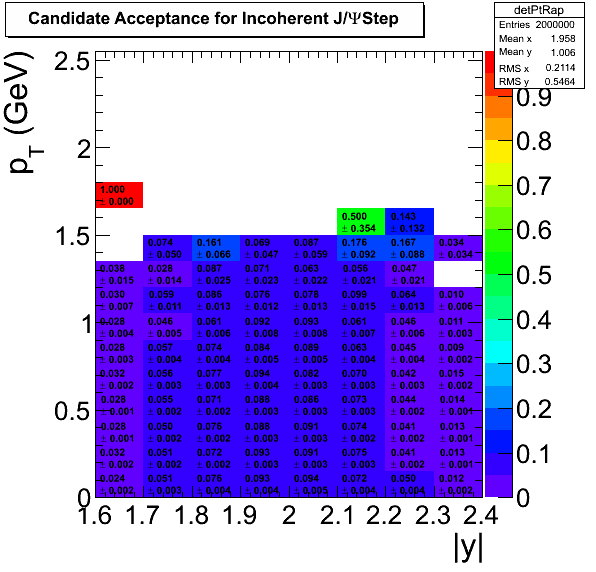
\includegraphics[width=.45\textwidth]{mcEffMaps/detAccJpInCoStep} \\
            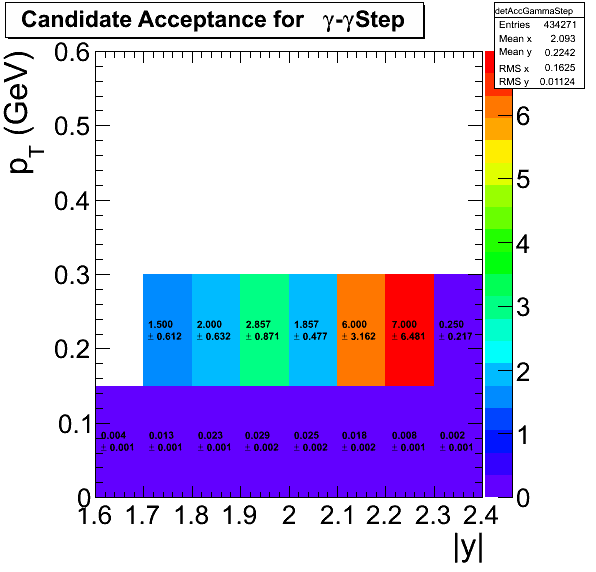
\includegraphics[width=.45\textwidth]{mcEffMaps/detAccGammaStep}
          \end{array} $
          \caption{Dimuon acceptance from coherent J/$\psi$ (top left), incoherent 
            J$\psi$ (top right), and photon-photon interactions (lower).}
          \label{fig:jpsiAcceptance}
        \end{figure*}



